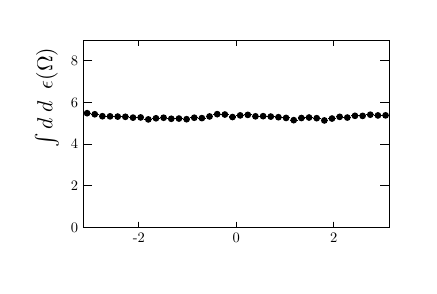
\begin{tikzpicture}
\pgfdeclareplotmark{cross} {
\pgfpathmoveto{\pgfpoint{-0.3\pgfplotmarksize}{\pgfplotmarksize}}
\pgfpathlineto{\pgfpoint{+0.3\pgfplotmarksize}{\pgfplotmarksize}}
\pgfpathlineto{\pgfpoint{+0.3\pgfplotmarksize}{0.3\pgfplotmarksize}}
\pgfpathlineto{\pgfpoint{+1\pgfplotmarksize}{0.3\pgfplotmarksize}}
\pgfpathlineto{\pgfpoint{+1\pgfplotmarksize}{-0.3\pgfplotmarksize}}
\pgfpathlineto{\pgfpoint{+0.3\pgfplotmarksize}{-0.3\pgfplotmarksize}}
\pgfpathlineto{\pgfpoint{+0.3\pgfplotmarksize}{-1.\pgfplotmarksize}}
\pgfpathlineto{\pgfpoint{-0.3\pgfplotmarksize}{-1.\pgfplotmarksize}}
\pgfpathlineto{\pgfpoint{-0.3\pgfplotmarksize}{-0.3\pgfplotmarksize}}
\pgfpathlineto{\pgfpoint{-1.\pgfplotmarksize}{-0.3\pgfplotmarksize}}
\pgfpathlineto{\pgfpoint{-1.\pgfplotmarksize}{0.3\pgfplotmarksize}}
\pgfpathlineto{\pgfpoint{-0.3\pgfplotmarksize}{0.3\pgfplotmarksize}}
\pgfpathclose
\pgfusepathqstroke
}
\pgfdeclareplotmark{cross*} {
\pgfpathmoveto{\pgfpoint{-0.3\pgfplotmarksize}{\pgfplotmarksize}}
\pgfpathlineto{\pgfpoint{+0.3\pgfplotmarksize}{\pgfplotmarksize}}
\pgfpathlineto{\pgfpoint{+0.3\pgfplotmarksize}{0.3\pgfplotmarksize}}
\pgfpathlineto{\pgfpoint{+1\pgfplotmarksize}{0.3\pgfplotmarksize}}
\pgfpathlineto{\pgfpoint{+1\pgfplotmarksize}{-0.3\pgfplotmarksize}}
\pgfpathlineto{\pgfpoint{+0.3\pgfplotmarksize}{-0.3\pgfplotmarksize}}
\pgfpathlineto{\pgfpoint{+0.3\pgfplotmarksize}{-1.\pgfplotmarksize}}
\pgfpathlineto{\pgfpoint{-0.3\pgfplotmarksize}{-1.\pgfplotmarksize}}
\pgfpathlineto{\pgfpoint{-0.3\pgfplotmarksize}{-0.3\pgfplotmarksize}}
\pgfpathlineto{\pgfpoint{-1.\pgfplotmarksize}{-0.3\pgfplotmarksize}}
\pgfpathlineto{\pgfpoint{-1.\pgfplotmarksize}{0.3\pgfplotmarksize}}
\pgfpathlineto{\pgfpoint{-0.3\pgfplotmarksize}{0.3\pgfplotmarksize}}
\pgfpathclose
\pgfusepathqfillstroke
}
\pgfdeclareplotmark{newstar} {
\pgfpathmoveto{\pgfqpoint{0pt}{\pgfplotmarksize}}
\pgfpathlineto{\pgfqpointpolar{44}{0.5\pgfplotmarksize}}
\pgfpathlineto{\pgfqpointpolar{18}{\pgfplotmarksize}}
\pgfpathlineto{\pgfqpointpolar{-20}{0.5\pgfplotmarksize}}
\pgfpathlineto{\pgfqpointpolar{-54}{\pgfplotmarksize}}
\pgfpathlineto{\pgfqpointpolar{-90}{0.5\pgfplotmarksize}}
\pgfpathlineto{\pgfqpointpolar{234}{\pgfplotmarksize}}
\pgfpathlineto{\pgfqpointpolar{198}{0.5\pgfplotmarksize}}
\pgfpathlineto{\pgfqpointpolar{162}{\pgfplotmarksize}}
\pgfpathlineto{\pgfqpointpolar{134}{0.5\pgfplotmarksize}}
\pgfpathclose
\pgfusepathqstroke
}
\pgfdeclareplotmark{newstar*} {
\pgfpathmoveto{\pgfqpoint{0pt}{\pgfplotmarksize}}
\pgfpathlineto{\pgfqpointpolar{44}{0.5\pgfplotmarksize}}
\pgfpathlineto{\pgfqpointpolar{18}{\pgfplotmarksize}}
\pgfpathlineto{\pgfqpointpolar{-20}{0.5\pgfplotmarksize}}
\pgfpathlineto{\pgfqpointpolar{-54}{\pgfplotmarksize}}
\pgfpathlineto{\pgfqpointpolar{-90}{0.5\pgfplotmarksize}}
\pgfpathlineto{\pgfqpointpolar{234}{\pgfplotmarksize}}
\pgfpathlineto{\pgfqpointpolar{198}{0.5\pgfplotmarksize}}
\pgfpathlineto{\pgfqpointpolar{162}{\pgfplotmarksize}}
\pgfpathlineto{\pgfqpointpolar{134}{0.5\pgfplotmarksize}}
\pgfpathclose
\pgfusepathqfillstroke
}
\definecolor{c}{rgb}{1,1,1};
\draw [color=c, fill=c] (0.1,0.0627517) rectangle (4.9,3.07483);
\draw [color=c, fill=c] (0.772,0.544685) rectangle (4.66,2.92423);
\definecolor{c}{rgb}{0,0,0};
\draw [c] (0.772,0.544685) -- (0.772,2.92423) -- (4.66,2.92423) -- (4.66,0.544685) -- (0.772,0.544685);
\draw [c,line width=0.4] (0.8206,1.98653) -- (0.8206,1.99592);
\draw [c,line width=0.4] (0.8206,1.99592) -- (0.8206,2.00531);
\draw [c,line width=0.4] (0.772,1.99592) -- (0.8206,1.99592);
\draw [c,line width=0.4] (0.8206,1.99592) -- (0.8692,1.99592);
\foreach \P in {(0.8206,1.99592)}{\draw[mark options={color=c,fill=c},mark size=2.402402pt,mark=*,mark size=1pt] plot coordinates {\P};}
\draw [c,line width=0.4] (0.9178,1.97266) -- (0.9178,1.982);
\draw [c,line width=0.4] (0.9178,1.982) -- (0.9178,1.99135);
\draw [c,line width=0.4] (0.8692,1.982) -- (0.9178,1.982);
\draw [c,line width=0.4] (0.9178,1.982) -- (0.9664,1.982);
\foreach \P in {(0.9178,1.982)}{\draw[mark options={color=c,fill=c},mark size=2.402402pt,mark=*,mark size=1pt] plot coordinates {\P};}
\draw [c,line width=0.4] (1.015,1.94805) -- (1.015,1.95731);
\draw [c,line width=0.4] (1.015,1.95731) -- (1.015,1.96658);
\draw [c,line width=0.4] (0.9664,1.95731) -- (1.015,1.95731);
\draw [c,line width=0.4] (1.015,1.95731) -- (1.0636,1.95731);
\foreach \P in {(1.015,1.95731)}{\draw[mark options={color=c,fill=c},mark size=2.402402pt,mark=*,mark size=1pt] plot coordinates {\P};}
\draw [c,line width=0.4] (1.1122,1.94635) -- (1.1122,1.9556);
\draw [c,line width=0.4] (1.1122,1.9556) -- (1.1122,1.96486);
\draw [c,line width=0.4] (1.0636,1.9556) -- (1.1122,1.9556);
\draw [c,line width=0.4] (1.1122,1.9556) -- (1.1608,1.9556);
\foreach \P in {(1.1122,1.9556)}{\draw[mark options={color=c,fill=c},mark size=2.402402pt,mark=*,mark size=1pt] plot coordinates {\P};}
\draw [c,line width=0.4] (1.2094,1.94343) -- (1.2094,1.95268);
\draw [c,line width=0.4] (1.2094,1.95268) -- (1.2094,1.96192);
\draw [c,line width=0.4] (1.1608,1.95268) -- (1.2094,1.95268);
\draw [c,line width=0.4] (1.2094,1.95268) -- (1.258,1.95268);
\foreach \P in {(1.2094,1.95268)}{\draw[mark options={color=c,fill=c},mark size=2.402402pt,mark=*,mark size=1pt] plot coordinates {\P};}
\draw [c,line width=0.4] (1.3066,1.94072) -- (1.3066,1.94996);
\draw [c,line width=0.4] (1.3066,1.94996) -- (1.3066,1.9592);
\draw [c,line width=0.4] (1.258,1.94996) -- (1.3066,1.94996);
\draw [c,line width=0.4] (1.3066,1.94996) -- (1.3552,1.94996);
\foreach \P in {(1.3066,1.94996)}{\draw[mark options={color=c,fill=c},mark size=2.402402pt,mark=*,mark size=1pt] plot coordinates {\P};}
\draw [c,line width=0.4] (1.4038,1.93026) -- (1.4038,1.93947);
\draw [c,line width=0.4] (1.4038,1.93947) -- (1.4038,1.94867);
\draw [c,line width=0.4] (1.3552,1.93947) -- (1.4038,1.93947);
\draw [c,line width=0.4] (1.4038,1.93947) -- (1.4524,1.93947);
\foreach \P in {(1.4038,1.93947)}{\draw[mark options={color=c,fill=c},mark size=2.402402pt,mark=*,mark size=1pt] plot coordinates {\P};}
\draw [c,line width=0.4] (1.501,1.93278) -- (1.501,1.94199);
\draw [c,line width=0.4] (1.501,1.94199) -- (1.501,1.9512);
\draw [c,line width=0.4] (1.4524,1.94199) -- (1.501,1.94199);
\draw [c,line width=0.4] (1.501,1.94199) -- (1.5496,1.94199);
\foreach \P in {(1.501,1.94199)}{\draw[mark options={color=c,fill=c},mark size=2.402402pt,mark=*,mark size=1pt] plot coordinates {\P};}
\draw [c,line width=0.4] (1.5982,1.9078) -- (1.5982,1.91693);
\draw [c,line width=0.4] (1.5982,1.91693) -- (1.5982,1.92606);
\draw [c,line width=0.4] (1.5496,1.91693) -- (1.5982,1.91693);
\draw [c,line width=0.4] (1.5982,1.91693) -- (1.6468,1.91693);
\foreach \P in {(1.5982,1.91693)}{\draw[mark options={color=c,fill=c},mark size=2.402402pt,mark=*,mark size=1pt] plot coordinates {\P};}
\draw [c,line width=0.4] (1.6954,1.922) -- (1.6954,1.93118);
\draw [c,line width=0.4] (1.6954,1.93118) -- (1.6954,1.94036);
\draw [c,line width=0.4] (1.6468,1.93118) -- (1.6954,1.93118);
\draw [c,line width=0.4] (1.6954,1.93118) -- (1.744,1.93118);
\foreach \P in {(1.6954,1.93118)}{\draw[mark options={color=c,fill=c},mark size=2.402402pt,mark=*,mark size=1pt] plot coordinates {\P};}
\draw [c,line width=0.4] (1.7926,1.92905) -- (1.7926,1.93825);
\draw [c,line width=0.4] (1.7926,1.93825) -- (1.7926,1.94746);
\draw [c,line width=0.4] (1.744,1.93825) -- (1.7926,1.93825);
\draw [c,line width=0.4] (1.7926,1.93825) -- (1.8412,1.93825);
\foreach \P in {(1.7926,1.93825)}{\draw[mark options={color=c,fill=c},mark size=2.402402pt,mark=*,mark size=1pt] plot coordinates {\P};}
\draw [c,line width=0.4] (1.8898,1.91573) -- (1.8898,1.92489);
\draw [c,line width=0.4] (1.8898,1.92489) -- (1.8898,1.93405);
\draw [c,line width=0.4] (1.8412,1.92489) -- (1.8898,1.92489);
\draw [c,line width=0.4] (1.8898,1.92489) -- (1.9384,1.92489);
\foreach \P in {(1.8898,1.92489)}{\draw[mark options={color=c,fill=c},mark size=2.402402pt,mark=*,mark size=1pt] plot coordinates {\P};}
\draw [c,line width=0.4] (1.987,1.91853) -- (1.987,1.9277);
\draw [c,line width=0.4] (1.987,1.9277) -- (1.987,1.93687);
\draw [c,line width=0.4] (1.9384,1.9277) -- (1.987,1.9277);
\draw [c,line width=0.4] (1.987,1.9277) -- (2.0356,1.9277);
\foreach \P in {(1.987,1.9277)}{\draw[mark options={color=c,fill=c},mark size=2.402402pt,mark=*,mark size=1pt] plot coordinates {\P};}
\draw [c,line width=0.4] (2.0842,1.91024) -- (2.0842,1.91938);
\draw [c,line width=0.4] (2.0842,1.91938) -- (2.0842,1.92852);
\draw [c,line width=0.4] (2.0356,1.91938) -- (2.0842,1.91938);
\draw [c,line width=0.4] (2.0842,1.91938) -- (2.1328,1.91938);
\foreach \P in {(2.0842,1.91938)}{\draw[mark options={color=c,fill=c},mark size=2.402402pt,mark=*,mark size=1pt] plot coordinates {\P};}
\draw [c,line width=0.4] (2.1814,1.92902) -- (2.1814,1.93822);
\draw [c,line width=0.4] (2.1814,1.93822) -- (2.1814,1.94742);
\draw [c,line width=0.4] (2.1328,1.93822) -- (2.1814,1.93822);
\draw [c,line width=0.4] (2.1814,1.93822) -- (2.23,1.93822);
\foreach \P in {(2.1814,1.93822)}{\draw[mark options={color=c,fill=c},mark size=2.402402pt,mark=*,mark size=1pt] plot coordinates {\P};}
\draw [c,line width=0.4] (2.2786,1.92407) -- (2.2786,1.93325);
\draw [c,line width=0.4] (2.2786,1.93325) -- (2.2786,1.94244);
\draw [c,line width=0.4] (2.23,1.93325) -- (2.2786,1.93325);
\draw [c,line width=0.4] (2.2786,1.93325) -- (2.3272,1.93325);
\foreach \P in {(2.2786,1.93325)}{\draw[mark options={color=c,fill=c},mark size=2.402402pt,mark=*,mark size=1pt] plot coordinates {\P};}
\draw [c,line width=0.4] (2.3758,1.94534) -- (2.3758,1.95459);
\draw [c,line width=0.4] (2.3758,1.95459) -- (2.3758,1.96385);
\draw [c,line width=0.4] (2.3272,1.95459) -- (2.3758,1.95459);
\draw [c,line width=0.4] (2.3758,1.95459) -- (2.4244,1.95459);
\foreach \P in {(2.3758,1.95459)}{\draw[mark options={color=c,fill=c},mark size=2.402402pt,mark=*,mark size=1pt] plot coordinates {\P};}
\draw [c,line width=0.4] (2.473,1.97421) -- (2.473,1.98356);
\draw [c,line width=0.4] (2.473,1.98356) -- (2.473,1.99291);
\draw [c,line width=0.4] (2.4244,1.98356) -- (2.473,1.98356);
\draw [c,line width=0.4] (2.473,1.98356) -- (2.5216,1.98356);
\foreach \P in {(2.473,1.98356)}{\draw[mark options={color=c,fill=c},mark size=2.402402pt,mark=*,mark size=1pt] plot coordinates {\P};}
\draw [c,line width=0.4] (2.5702,1.96938) -- (2.5702,1.97871);
\draw [c,line width=0.4] (2.5702,1.97871) -- (2.5702,1.98805);
\draw [c,line width=0.4] (2.5216,1.97871) -- (2.5702,1.97871);
\draw [c,line width=0.4] (2.5702,1.97871) -- (2.6188,1.97871);
\foreach \P in {(2.5702,1.97871)}{\draw[mark options={color=c,fill=c},mark size=2.402402pt,mark=*,mark size=1pt] plot coordinates {\P};}
\draw [c,line width=0.4] (2.6674,1.93764) -- (2.6674,1.94687);
\draw [c,line width=0.4] (2.6674,1.94687) -- (2.6674,1.9561);
\draw [c,line width=0.4] (2.6188,1.94687) -- (2.6674,1.94687);
\draw [c,line width=0.4] (2.6674,1.94687) -- (2.716,1.94687);
\foreach \P in {(2.6674,1.94687)}{\draw[mark options={color=c,fill=c},mark size=2.402402pt,mark=*,mark size=1pt] plot coordinates {\P};}
\draw [c,line width=0.4] (2.7646,1.9586) -- (2.7646,1.9679);
\draw [c,line width=0.4] (2.7646,1.9679) -- (2.7646,1.9772);
\draw [c,line width=0.4] (2.716,1.9679) -- (2.7646,1.9679);
\draw [c,line width=0.4] (2.7646,1.9679) -- (2.8132,1.9679);
\foreach \P in {(2.7646,1.9679)}{\draw[mark options={color=c,fill=c},mark size=2.402402pt,mark=*,mark size=1pt] plot coordinates {\P};}
\draw [c,line width=0.4] (2.8618,1.96503) -- (2.8618,1.97435);
\draw [c,line width=0.4] (2.8618,1.97435) -- (2.8618,1.98367);
\draw [c,line width=0.4] (2.8132,1.97435) -- (2.8618,1.97435);
\draw [c,line width=0.4] (2.8618,1.97435) -- (2.9104,1.97435);
\foreach \P in {(2.8618,1.97435)}{\draw[mark options={color=c,fill=c},mark size=2.402402pt,mark=*,mark size=1pt] plot coordinates {\P};}
\draw [c,line width=0.4] (2.959,1.94673) -- (2.959,1.95599);
\draw [c,line width=0.4] (2.959,1.95599) -- (2.959,1.96525);
\draw [c,line width=0.4] (2.9104,1.95599) -- (2.959,1.95599);
\draw [c,line width=0.4] (2.959,1.95599) -- (3.0076,1.95599);
\foreach \P in {(2.959,1.95599)}{\draw[mark options={color=c,fill=c},mark size=2.402402pt,mark=*,mark size=1pt] plot coordinates {\P};}
\draw [c,line width=0.4] (3.0562,1.9488) -- (3.0562,1.95807);
\draw [c,line width=0.4] (3.0562,1.95807) -- (3.0562,1.96733);
\draw [c,line width=0.4] (3.0076,1.95807) -- (3.0562,1.95807);
\draw [c,line width=0.4] (3.0562,1.95807) -- (3.1048,1.95807);
\foreach \P in {(3.0562,1.95807)}{\draw[mark options={color=c,fill=c},mark size=2.402402pt,mark=*,mark size=1pt] plot coordinates {\P};}
\draw [c,line width=0.4] (3.1534,1.94343) -- (3.1534,1.95268);
\draw [c,line width=0.4] (3.1534,1.95268) -- (3.1534,1.96193);
\draw [c,line width=0.4] (3.1048,1.95268) -- (3.1534,1.95268);
\draw [c,line width=0.4] (3.1534,1.95268) -- (3.202,1.95268);
\foreach \P in {(3.1534,1.95268)}{\draw[mark options={color=c,fill=c},mark size=2.402402pt,mark=*,mark size=1pt] plot coordinates {\P};}
\draw [c,line width=0.4] (3.2506,1.93572) -- (3.2506,1.94495);
\draw [c,line width=0.4] (3.2506,1.94495) -- (3.2506,1.95417);
\draw [c,line width=0.4] (3.202,1.94495) -- (3.2506,1.94495);
\draw [c,line width=0.4] (3.2506,1.94495) -- (3.2992,1.94495);
\foreach \P in {(3.2506,1.94495)}{\draw[mark options={color=c,fill=c},mark size=2.402402pt,mark=*,mark size=1pt] plot coordinates {\P};}
\draw [c,line width=0.4] (3.3478,1.92627) -- (3.3478,1.93546);
\draw [c,line width=0.4] (3.3478,1.93546) -- (3.3478,1.94465);
\draw [c,line width=0.4] (3.2992,1.93546) -- (3.3478,1.93546);
\draw [c,line width=0.4] (3.3478,1.93546) -- (3.3964,1.93546);
\foreach \P in {(3.3478,1.93546)}{\draw[mark options={color=c,fill=c},mark size=2.402402pt,mark=*,mark size=1pt] plot coordinates {\P};}
\draw [c,line width=0.4] (3.445,1.8983) -- (3.445,1.9074);
\draw [c,line width=0.4] (3.445,1.9074) -- (3.445,1.91649);
\draw [c,line width=0.4] (3.3964,1.9074) -- (3.445,1.9074);
\draw [c,line width=0.4] (3.445,1.9074) -- (3.4936,1.9074);
\foreach \P in {(3.445,1.9074)}{\draw[mark options={color=c,fill=c},mark size=2.402402pt,mark=*,mark size=1pt] plot coordinates {\P};}
\draw [c,line width=0.4] (3.5422,1.9253) -- (3.5422,1.93448);
\draw [c,line width=0.4] (3.5422,1.93448) -- (3.5422,1.94367);
\draw [c,line width=0.4] (3.4936,1.93448) -- (3.5422,1.93448);
\draw [c,line width=0.4] (3.5422,1.93448) -- (3.5908,1.93448);
\foreach \P in {(3.5422,1.93448)}{\draw[mark options={color=c,fill=c},mark size=2.402402pt,mark=*,mark size=1pt] plot coordinates {\P};}
\draw [c,line width=0.4] (3.6394,1.93164) -- (3.6394,1.94085);
\draw [c,line width=0.4] (3.6394,1.94085) -- (3.6394,1.95006);
\draw [c,line width=0.4] (3.5908,1.94085) -- (3.6394,1.94085);
\draw [c,line width=0.4] (3.6394,1.94085) -- (3.688,1.94085);
\foreach \P in {(3.6394,1.94085)}{\draw[mark options={color=c,fill=c},mark size=2.402402pt,mark=*,mark size=1pt] plot coordinates {\P};}
\draw [c,line width=0.4] (3.7366,1.92319) -- (3.7366,1.93238);
\draw [c,line width=0.4] (3.7366,1.93238) -- (3.7366,1.94156);
\draw [c,line width=0.4] (3.688,1.93238) -- (3.7366,1.93238);
\draw [c,line width=0.4] (3.7366,1.93238) -- (3.7852,1.93238);
\foreach \P in {(3.7366,1.93238)}{\draw[mark options={color=c,fill=c},mark size=2.402402pt,mark=*,mark size=1pt] plot coordinates {\P};}
\draw [c,line width=0.4] (3.8338,1.89466) -- (3.8338,1.90375);
\draw [c,line width=0.4] (3.8338,1.90375) -- (3.8338,1.91283);
\draw [c,line width=0.4] (3.7852,1.90375) -- (3.8338,1.90375);
\draw [c,line width=0.4] (3.8338,1.90375) -- (3.8824,1.90375);
\foreach \P in {(3.8338,1.90375)}{\draw[mark options={color=c,fill=c},mark size=2.402402pt,mark=*,mark size=1pt] plot coordinates {\P};}
\draw [c,line width=0.4] (3.931,1.91882) -- (3.931,1.92799);
\draw [c,line width=0.4] (3.931,1.92799) -- (3.931,1.93716);
\draw [c,line width=0.4] (3.8824,1.92799) -- (3.931,1.92799);
\draw [c,line width=0.4] (3.931,1.92799) -- (3.9796,1.92799);
\foreach \P in {(3.931,1.92799)}{\draw[mark options={color=c,fill=c},mark size=2.402402pt,mark=*,mark size=1pt] plot coordinates {\P};}
\draw [c,line width=0.4] (4.0282,1.94005) -- (4.0282,1.94929);
\draw [c,line width=0.4] (4.0282,1.94929) -- (4.0282,1.95853);
\draw [c,line width=0.4] (3.9796,1.94929) -- (4.0282,1.94929);
\draw [c,line width=0.4] (4.0282,1.94929) -- (4.0768,1.94929);
\foreach \P in {(4.0282,1.94929)}{\draw[mark options={color=c,fill=c},mark size=2.402402pt,mark=*,mark size=1pt] plot coordinates {\P};}
\draw [c,line width=0.4] (4.1254,1.93127) -- (4.1254,1.94048);
\draw [c,line width=0.4] (4.1254,1.94048) -- (4.1254,1.94969);
\draw [c,line width=0.4] (4.0768,1.94048) -- (4.1254,1.94048);
\draw [c,line width=0.4] (4.1254,1.94048) -- (4.174,1.94048);
\foreach \P in {(4.1254,1.94048)}{\draw[mark options={color=c,fill=c},mark size=2.402402pt,mark=*,mark size=1pt] plot coordinates {\P};}
\draw [c,line width=0.4] (4.2226,1.95317) -- (4.2226,1.96245);
\draw [c,line width=0.4] (4.2226,1.96245) -- (4.2226,1.97173);
\draw [c,line width=0.4] (4.174,1.96245) -- (4.2226,1.96245);
\draw [c,line width=0.4] (4.2226,1.96245) -- (4.2712,1.96245);
\foreach \P in {(4.2226,1.96245)}{\draw[mark options={color=c,fill=c},mark size=2.402402pt,mark=*,mark size=1pt] plot coordinates {\P};}
\draw [c,line width=0.4] (4.3198,1.95225) -- (4.3198,1.96153);
\draw [c,line width=0.4] (4.3198,1.96153) -- (4.3198,1.9708);
\draw [c,line width=0.4] (4.2712,1.96153) -- (4.3198,1.96153);
\draw [c,line width=0.4] (4.3198,1.96153) -- (4.3684,1.96153);
\foreach \P in {(4.3198,1.96153)}{\draw[mark options={color=c,fill=c},mark size=2.402402pt,mark=*,mark size=1pt] plot coordinates {\P};}
\draw [c,line width=0.4] (4.417,1.96738) -- (4.417,1.97671);
\draw [c,line width=0.4] (4.417,1.97671) -- (4.417,1.98603);
\draw [c,line width=0.4] (4.3684,1.97671) -- (4.417,1.97671);
\draw [c,line width=0.4] (4.417,1.97671) -- (4.4656,1.97671);
\foreach \P in {(4.417,1.97671)}{\draw[mark options={color=c,fill=c},mark size=2.402402pt,mark=*,mark size=1pt] plot coordinates {\P};}
\draw [c,line width=0.4] (4.5142,1.95805) -- (4.5142,1.96735);
\draw [c,line width=0.4] (4.5142,1.96735) -- (4.5142,1.97665);
\draw [c,line width=0.4] (4.4656,1.96735) -- (4.5142,1.96735);
\draw [c,line width=0.4] (4.5142,1.96735) -- (4.5628,1.96735);
\foreach \P in {(4.5142,1.96735)}{\draw[mark options={color=c,fill=c},mark size=2.402402pt,mark=*,mark size=1pt] plot coordinates {\P};}
\draw [c,line width=0.4] (4.6114,1.95904) -- (4.6114,1.96834);
\draw [c,line width=0.4] (4.6114,1.96834) -- (4.6114,1.97764);
\draw [c,line width=0.4] (4.5628,1.96834) -- (4.6114,1.96834);
\draw [c,line width=0.4] (4.6114,1.96834) -- (4.66,1.96834);
\foreach \P in {(4.6114,1.96834)}{\draw[mark options={color=c,fill=c},mark size=2.402402pt,mark=*,mark size=1pt] plot coordinates {\P};}
\draw [c,line width=0.4] (0.772,0.544685) -- (4.66,0.544685);
\draw [anchor= east] (4.66,0.255525) node[scale=0.78483, rotate=0]{$\phihel$};
\draw [c,line width=0.4] (1.47778,0.617878) -- (1.47778,0.544685);
\draw [c,line width=0.4] (2.716,0.617878) -- (2.716,0.544685);
\draw [c,line width=0.4] (3.95422,0.617878) -- (3.95422,0.544685);
\draw [c,line width=0.4] (1.47778,0.617878) -- (1.47778,0.544685);
\draw [c,line width=0.4] (3.95422,0.617878) -- (3.95422,0.544685);
\draw [anchor=base] (1.47778,0.351911) node[scale=0.52322, rotate=0]{-2};
\draw [anchor=base] (2.716,0.351911) node[scale=0.52322, rotate=0]{0};
\draw [anchor=base] (3.95422,0.351911) node[scale=0.52322, rotate=0]{2};
\draw [c,line width=0.4] (0.772,2.92423) -- (4.66,2.92423);
\draw [c,line width=0.4] (1.47778,2.85103) -- (1.47778,2.92423);
\draw [c,line width=0.4] (2.716,2.85103) -- (2.716,2.92423);
\draw [c,line width=0.4] (3.95422,2.85103) -- (3.95422,2.92423);
\draw [c,line width=0.4] (1.47778,2.85103) -- (1.47778,2.92423);
\draw [c,line width=0.4] (3.95422,2.85103) -- (3.95422,2.92423);
\draw [c,line width=0.4] (0.772,0.544685) -- (0.772,2.92423);
\draw [anchor= east] (0.3112,2.92423) node[scale=0.78483, rotate=90]{$\int d\thetaK \; d\thetamu \;\; \epsilon(\Omega) $};
\draw [c,line width=0.4] (0.88576,0.544685) -- (0.772,0.544685);
\draw [c,line width=0.4] (0.88576,1.07347) -- (0.772,1.07347);
\draw [c,line width=0.4] (0.88576,1.60226) -- (0.772,1.60226);
\draw [c,line width=0.4] (0.88576,2.13105) -- (0.772,2.13105);
\draw [c,line width=0.4] (0.88576,2.65983) -- (0.772,2.65983);
\draw [c,line width=0.4] (0.88576,2.65983) -- (0.772,2.65983);
\draw [anchor= east] (0.772,0.544685) node[scale=0.52322, rotate=0]{0};
\draw [anchor= east] (0.772,1.07347) node[scale=0.52322, rotate=0]{2};
\draw [anchor= east] (0.772,1.60226) node[scale=0.52322, rotate=0]{4};
\draw [anchor= east] (0.772,2.13105) node[scale=0.52322, rotate=0]{6};
\draw [anchor= east] (0.772,2.65983) node[scale=0.52322, rotate=0]{8};
\draw [c,line width=0.4] (4.66,0.544685) -- (4.66,2.92423);
\draw [c,line width=0.4] (4.54624,0.544685) -- (4.66,0.544685);
\draw [c,line width=0.4] (4.54624,1.07347) -- (4.66,1.07347);
\draw [c,line width=0.4] (4.54624,1.60226) -- (4.66,1.60226);
\draw [c,line width=0.4] (4.54624,2.13105) -- (4.66,2.13105);
\draw [c,line width=0.4] (4.54624,2.65983) -- (4.66,2.65983);
\draw [c,line width=0.4] (4.54624,2.65983) -- (4.66,2.65983);
\end{tikzpicture}
